% Author: Izaak Neutelings (November 2020)
\documentclass[border=3pt,tikz]{standalone}
\usepackage{siunitx}
%\usepackage{physics}
\usepackage{tikz}
%\usepackage[outline]{contour} % glow around text
\usetikzlibrary{patterns,decorations.pathmorphing}
\usetikzlibrary{arrows.meta}
\tikzset{>=latex}
%\contourlength{1.1pt}

\colorlet{mydarkblue}{blue!50!black}
\colorlet{myred}{red!65!black}
\tikzstyle{force}=[->,myred,very thick,line cap=round]
\tikzstyle{vvec}=[->,very thick,vcol,line cap=round]
\def\tick#1#2{\draw[thick] (#1)++(#2:0.1) --++ (#2-180:0.2)}

\begin{document}


% ATMOSPHERIC PRESSURE vs. ALTITUDE
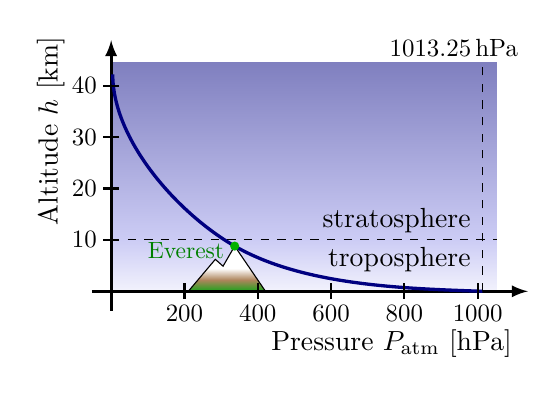
\begin{tikzpicture}
  \def\xmax{4.9}
  \def\ymax{2.9}
  \def\Nx{5}
  \def\Ny{4}
  \coordinate (M) at (0.95*\xmax*3.37/2/\Nx,0.9*\ymax*0.88/\Ny); % mount Everest
  \coordinate (S) at (0.95*\xmax*10.13/2/\Nx,0); % sea level
  
  % SKY + MOUNTAIN
  \fill[top color=blue!80!black!20,bottom color=blue!80!black!5]
    (0,0) rectangle (\xmax,0.9/\Ny*\ymax);
  \fill[top color=blue!50!black!50,bottom color=blue!80!black!20]
    (0,0.9/\Ny*\ymax) rectangle (\xmax,\ymax);
  \begin{scope}
    \clip (0.2*\xmax,0) --++ (0.07*\xmax,0.14*\ymax) --++ (0.02*\xmax,-0.03*\ymax) -- (M) -- (0.4*\xmax,0);
    \fill[white] (0.1*\xmax,0) rectangle (0.4*\xmax,0.5*\ymax);
    \fill[top color=white,bottom color=green!60!black!90,middle color=brown!80!black!80]
      (0.1*\xmax,0) rectangle (0.4*\xmax,0.1*\ymax);
  \end{scope}
  \draw[thin] (0.2*\xmax,0) --++ (0.07*\xmax,0.14*\ymax) --++ (0.02*\xmax,-0.03*\ymax) -- (M) -- (0.4*\xmax,0);
  
  % AXES
  \draw[->,line width=1] (-0.05*\xmax,0) -- (1.08*\xmax,0) node[right=8,below left=10] {Pressure $P_\mathrm{atm}$ [hPa]};
  \draw[->,line width=1] (0,-0.05*\xmax) -- (0,1.10*\ymax) node[below=8,above left=13,rotate=90] {Altitude $h$ [km]};
  
  % LINE
  \draw[mydarkblue,very thick]
    (0.02,0.95*\ymax) to[out=-90,in=150,looseness=0.8]
    (M) to[out=-30,in=178,looseness=0.8] (S);
  \fill[green!70!black] (M) circle(0.02*\ymax) node[green!50!black,below=1.7,left=0.8,scale=0.85] {Everest};
  
  % TICKS
  \foreach \i [evaluate={\y=0.9*\ymax*\i/\Ny; \h=int(10*\i)}] in {1,...,\Ny}{
    \tick{0,\y}{0} node[left=-1,scale=0.9] {\h};
  }
  \foreach \i [evaluate={\x=0.95*\xmax*\i/\Nx; \p=int(200*\i)}] in {1,...,\Nx}{
    \tick{\x,0}{90} node[below=-1,scale=0.9] {\p};
  }
  \draw[dashed]
    (0,0.9/\Ny*\ymax) --++ (\xmax,0)
    node[left=7,below left=-1] {troposphere}
    node[left=7,above left=-1] {stratosphere};
  \draw[dashed]
    (S) --++ (0,\ymax) % --++ (0,0.05*\ymax) (S)++(0,0.2*\ymax) --++ (0,0.8*\ymax)
    node[right=15,above left=-1,scale=0.9] {\SI{1013.25}{hPa}};
\end{tikzpicture}


% ATMOSPHERIC PRESSURE vs. ALTITUDE - gas molecules
% Inverse transform sampling:
%   pdf f(x) = a*exp(-ax) => cdf F(x) = 1-exp(-ax)
%                         => F^{-1}(x) = -ln(1-x)/a
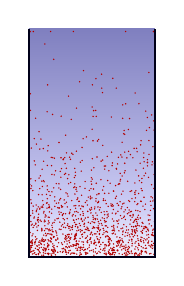
\begin{tikzpicture}
  \def\xmax{1.6}
  \def\ymax{2.9}
  \def\a{6}    % exponential rate parameter
  \def\N{1200} % number of particles
  \def\Ny{4}
  \fill[top color=blue!80!black!20,bottom color=blue!80!black!5]
    (0,0) rectangle (\xmax,0.9/\Ny*\ymax);
  \fill[top color=blue!50!black!50,bottom color=blue!80!black!20]
    (0,0.9/\Ny*\ymax) rectangle (\xmax,\ymax);
  \foreach \i [evaluate={\x=\xmax*(rand+1)/2;\y=0.008*\ymax+\ymax*min(0.98,-ln(1-(rand+1)/2)/\a);}] in {1,...,\N}{
    \fill[red!70!black] (\x,\y) circle(0.01);
  }
  \draw[thick,black!90!blue] (0,\ymax) -- (0,0) -- (\xmax,0) -- (\xmax,\ymax);
\end{tikzpicture}


\end{document}
